\documentclass[10pt,conference,compsocconf]{IEEEtran}
\setlength\parindent{0pt}
\usepackage{mathtools}
\usepackage{hyperref}
\usepackage{graphicx}	% For figure environment
\usepackage{subcaption}

\usepackage{listings}
\usepackage{xcolor}

\definecolor{codegreen}{rgb}{0,0.6,0}
\definecolor{codegray}{rgb}{0.5,0.5,0.5}
\definecolor{codepurple}{rgb}{0.58,0,0.82}
\definecolor{backcolour}{rgb}{0.95,0.95,0.92}

\lstdefinestyle{mystyle}{
    backgroundcolor=\color{backcolour},   
    commentstyle=\color{codegreen},
    keywordstyle=\color{magenta},
    numberstyle=\tiny\color{codegray},
    stringstyle=\color{codepurple},
    basicstyle=\ttfamily\footnotesize,
    breakatwhitespace=false,         
    breaklines=true,                 
    captionpos=b,                    
    keepspaces=true,                 
    numbers=left,                    
    numbersep=5pt,                  
    showspaces=false,                
    showstringspaces=false,
    showtabs=false,                  
    tabsize=2
}

\lstset{style=mystyle}

\begin{document}
\title{Deep Learning Project 2: Report}

\author{
  Raphael Bonatti\\
  Lena Csomor\\
  Marijn van der Meer\\
  \textit{Department of Computer Science, EPF Lausanne, Switzerland}
}

\maketitle

\section{Introduction}\label{sec:introduction}
In the scope of this project, we implemented several popular Machine Learning modules and activation functions using only PyTorch's standard tensor operations and the math library. All modules run with \texttt{autograd} globally off. Overall, these modules were combined into a model trained on points sampled uniformly from $[0,1]^2$ with labels $1$ if they are within a disk centered at $(0.5, 0.5)$ with radius $r = 1/\sqrt{2\pi}$ and $0$ otherwise. We compared the performance of our architecture to the same model built with pre-implemented PyTorch modules.

\section{Modules implementation}
\label{sec:module-implementation}
For our implementations we used the structure suggested in the project description which is to define a
\texttt{Module} class and have all modules inherit from it. 

\lstinputlisting[language=Python]{module.m}


\subsection{Linear module}\label{subsec:linear}

The \texttt{Linear} module applies a linear transformation of the form $y=A^Tx
 +b$ to its input. For familiarity purposes, the signature of the \texttt{init} method is the same as the one in the PyTorch framework. It initialises all weights and bias vectors to values sampled uniformly between $[0,1]$. Our version of the linear module also has a bias flag, which corresponds to enabling or disabling the bias term. To update the module weights during training, we store the input, the weights and the gradients with respect to the parameters i.e., weight and bias. The input is stored during the forward pass so that it can be used in the backward pass to compute the gradient with respect to the weights. We can access the module's parameters (weight and bias) and its gradients with respect to the parameters by calling the \texttt{param()} method. This method returns a dictionary, whose values can be easily accessed with the keys \texttt{weight} and \texttt{grad}. For the purpose of our task, this module can also take a tuple as an input and it will output a tuple of the same size. In that case, a tuple  of gradients will also be stored.  
 
 
 
\subsection{Tanh module}
The \texttt{Tanh} module is an activation function that applies the tanh function element-wise to its input. It can be used as a replacement for the sigmoid activation function, as it outputs numbers in $[-1,1]$. This module does not have a \texttt{param()} method as it is an activation function and has no specific parameters. It also does not have weights that need to be updated. However, it still needs to store the input to compute the backward pass. Like the linear module, this module accepts tuples.

%\lstinputlisting[language=Python]{tanh.m}


\subsection{ReLU module}
The \texttt{ReLU} module applies a piece-wise linear ReLU function element-wise to its input. ReLU has become a popular activation function for especially MLPs and CNNs because it is supposed to overcome the vanishing gradient problem~\cite{relu}.
\begin{equation}
    f(x) = max(x, 0)
\end{equation}
\[ f'(x) =
    \begin{cases} 
      0 & x < 0 \\
      1 & 0\leq x 
    \end{cases}
\]
Similarly to \texttt{Tanh}, this module accepts tuples as well and does not have a \texttt{param()} method as it is an activation function. \texttt{ReLU} also stores the input to compute the backward pass.

%\lstinputlisting[language=Python]{relu.m}
\subsection{LeakyReLU module}
The \texttt{LeakyReLU} applies a parametric ReLU function to the input, also known as Leaky ReLU, which does not set the gradient to 0 for inactive units, but allows it to stay at a small, positive value. Its parameter $\alpha$ is usually chosen between 0 and 1. %Therefore, \texttt{LeakyReLU} also has a \texttt{param()} function that returns a list with the only element being $\alpha$. (I had to remove this for it to work in sequential because of a clause, :( it does not have a parameter function anymore). \\
The main idea of Leaky ReLU is to let the gradient be non zero and recover during training eventually, so that we ideally avoid a vanishing gradient problem. We decided to implement Leaky ReLU so that we could compare its effect on our model compared to standard ReLU.  
\begin{equation}
    f(x, \alpha) = max(x, \alpha*x)
\end{equation}
\[ f'(x) =
    \begin{cases} 
      \alpha & x < 0 \\
      1 & 0\leq x 
    \end{cases}
\]
\subsection{Sequential module}
The \texttt{Sequential} module is a container for sub-modules and allows us to assemble different modules and activation functions. It adds the modules passed to the constructor in the same order to the model. The \texttt{Sequential} module feeds the outputs of sub-modules as inputs to the next sub-modules during forward pass and passes the gradients in the reverse order during backward propagation. The module also works for tuples as inputs. 

\lstinputlisting[language=Python]{sequential.m}

\section{The Model}
\label{sec:baseline-model}
For simplicity reasons and to be able to use the modules we had at hand, we implemented our task as a regression problem rather than classification. This was mainly motivated by the fact that we had to train our model with Mean Squared Error (MSE), which is usually considered as a bad choice for classification. Furthermore, this way there was no additional function needed like a sigmoid or softmax to transform output probabilities into a class. For further work, we would have implemented Binary Cross Entropy to be able to transform the task into classification. 


As instructed, we constructed a network with two input units, one output unit and three hidden layers of 25 units (Figure~\ref{fig:model}). As seen in Figure~\ref{fig:model}, we used ReLU (or Leaky ReLU) between the input layer and the first hidden layer. All other activation functions used were Tanh. We also tried another architecture where we changed the first ReLU to Tanh and a second architecture with more ReLU layers instead of Tanh. However, these models either gave worse performances or vanishing gradients. 



\begin{figure}[htbp]
  \centering
  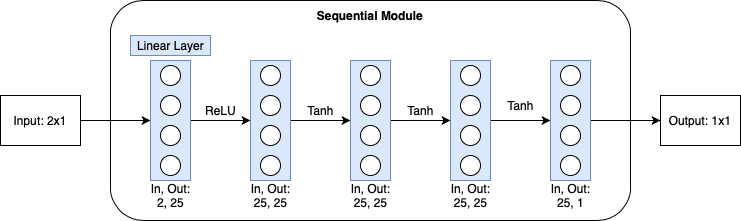
\includegraphics[width=\columnwidth]{doc/project2-report/model.png}
  \vspace{-3mm}
  \caption{Visualisation of Model constructed of submodules. The network has  two  input units,  one  output  unit  and  three  hidden  layers  of  25  units}
  \label{fig:model}
\end{figure}

\subsection{Training}\label{subsec:training}

This model was trained using mini-batch gradient descent with mini-batches of size 4 and a learning rate of $1e^{-4}$. As an optimiser, we implemented stochastic gradient descent (SGD) and gradient descent (GD) but chose to use GD for the final implementation to take advantage of using tuples of tensors to create mini-batches. We experimented with bigger batch sizes but the performance was poor, so we kept a small batch size. The test and training set were both of size 1000 and normalised using z-score normalisation. Results of the training and test loss can be seen in Figure~\ref{fig:relu}. The final training and test loss are $0.25048$. We see that both training and test loss are very close and that the model oscillates around a $0.25$ loss for the last iterations. 

\begin{figure}[t]
        \centering
        \begin{subfigure}[b]{\columnwidth}
            \centering 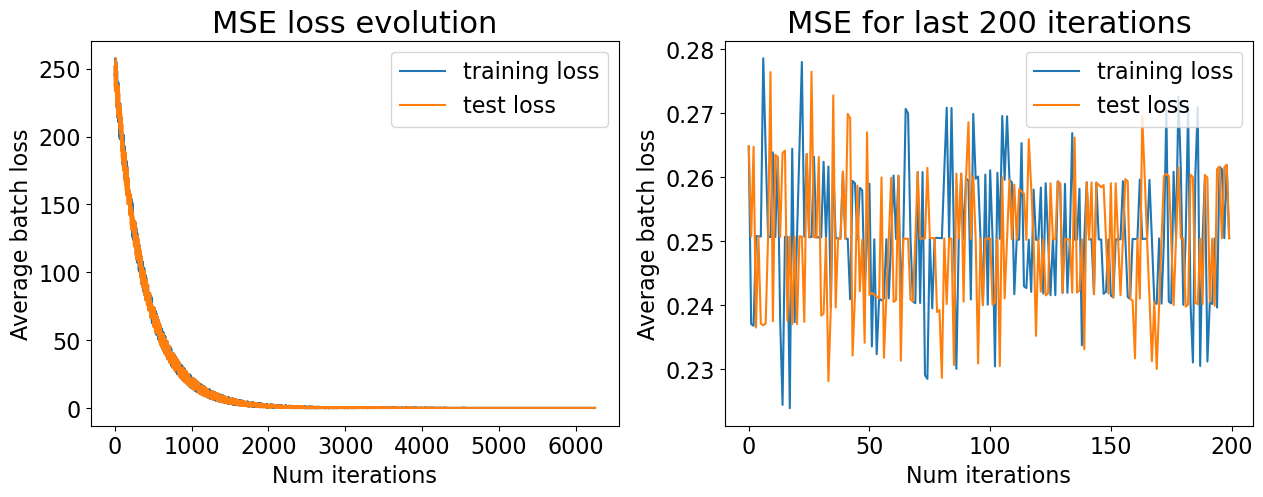
\includegraphics[width=\columnwidth]{doc/project2-report/Loss_project_2.png}
            \caption[]%
            {\small Model with ReLU.}   
     \label{fig:relu}
        \end{subfigure}
                \hfill 
        \begin{subfigure}[b]{\columnwidth}
            \centering 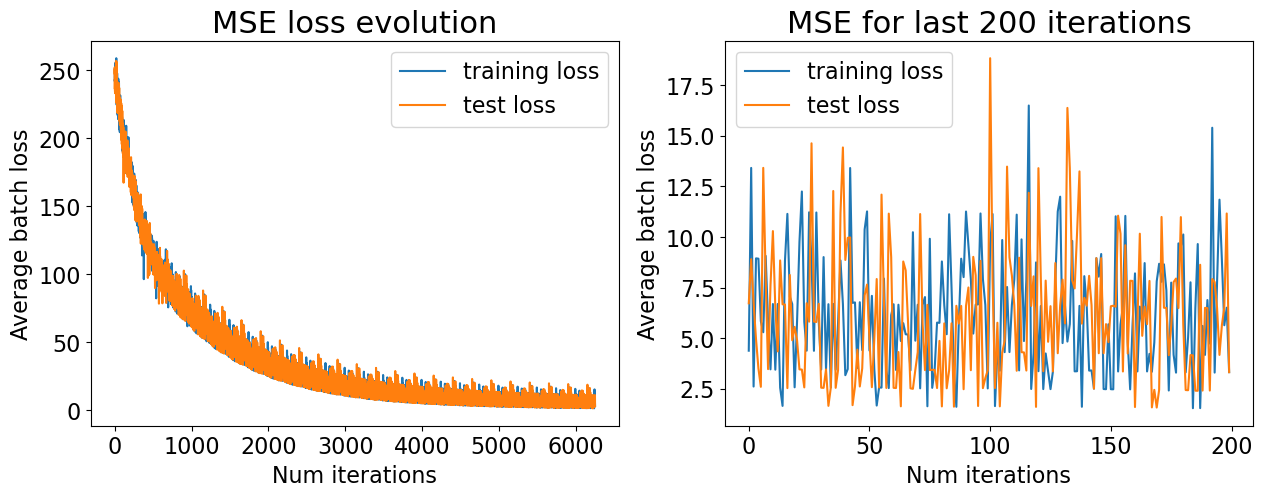
\includegraphics[width=\columnwidth]{doc/project2-report/Loss_project_2_leaky.png}
            \caption[]%
            {\small Model with Leaky ReLU.}     \label{fig:leaky-relu}
        \end{subfigure}
        \caption[]
        {Visualisation the evolution of the training (blue) and test MSE loss (orange) of model constructed with our sub-modules (Figure~\ref{fig:model}). On the left is the MSE loss over all iterations and on the right for the last 200 iterations. The number of iterations is given by the number of epochs (25) multiplied by the number of mini-batches created from the dataset (250).}
        \label{fig:loss-our-model}
    \end{figure}


We also trained a second model where we replaced the ReLU activation with a Leaky ReLU. But, as can be seen in Figure~\ref{fig:leaky-relu}, the performance is poorer for this activation function, with a final train and test loss of 3.32610. The amplitude of oscillations are also much bigger than for ReLU.  

\section{Comparison to PyTorch}
As a comparison, we created the same module with the pre-implemented PyTorch framework and trained it in the same way with MSE, a batch-size of 4 and learning rate of $1e^{-4}$. The only difference is that we had to use the SGD optimiser as normal GD, which is not implemented as an optimiser in PyTorch. But according to PyTorch documentation their SGD is actually a vanilla gradient descent. 

Unsurprisingly, the performance of this implementation is significantly better than our model (Figure~\ref{fig:model-pytorch}), with a final training and test loss of respectively 0.01765 and 0.01646. We also see that the model converges much faster and that there are almost no oscillations. We also notice that, like for our model, training and test losses are very close. 

We suspect that, though SGD is described as a vanilla gradient descent in the documentation, it might still be differently implemented than a simple gradient descent and be one of the reasons that this model performs better. Furthermore, PyTorch being a very popular and professional framework, it is highly probable that other internal implementation differences make their modules faster and better. 

\label{sec:improved-models}
\begin{figure}[htbp]
  \centering
  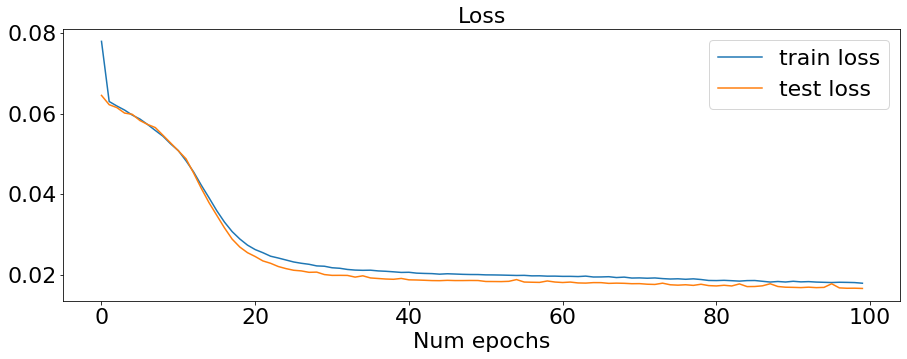
\includegraphics[width=\columnwidth]{doc/project2-report/mse_preimpl.png}
  \vspace{-3mm}
  \caption{Visualisation of MSE training (blue) and test loss (orange) evolution over 100 epochs using an architecture constructed with standard PyTorch modules.}
  \label{fig:model-pytorch}
\end{figure}

\section{Summary}
Overall, we created a model that performs a regression with a final loss of 0.25. To improve this and get closer to the loss of performance of the model that used official PyTorch modules, we could implement softmax and Binary Cross Entropy modules to formulate the task as classification. We could also implement different optimisers like Adam or SignSGD to aim to dampen oscillations and converge faster.


\bibliographystyle{IEEEtran}
\bibliography{literature}

\newpage

%\lstinputlisting[language=Python]{linear.m}
%\lstinputlisting[language=Python]{tanh.m}


\end{document}
